\documentclass[12pt]{article}

\usepackage{fontspec}
\usepackage{xeCJK}
\usepackage{amsmath,amssymb}
\usepackage{geometry}
\usepackage{array}
\usepackage{tikz}

\IfFontExistsTF{Songti SC}
    {\setCJKmainfont{Songti SC}}
    {\setCJKmainfont{FandolSong-Regular}}
\IfFontExistsTF{Heiti SC}
    {\setCJKsansfont{Heiti SC}}
    {\setCJKsansfont{FandolHei-Regular}}
\IfFontExistsTF{Songti SC}
    {\setCJKmonofont{Songti SC}}
    {\setCJKmonofont{FandolSong-Regular}}

\geometry{a4paper,margin=1in}
\renewcommand{\arraystretch}{1.25}
\setlength{\parindent}{2em}

\begin{document}

\begin{center}
    {\LARGE\bfseries 编译原理作业 3\par}
    \vspace{1.0cm}
    {\large
    \begin{tabular}{rl}
    姓名：& 梁力航 \\
    学号：& 23336128 \\
    日期：& 2026年5月7日
    \end{tabular}\par}
\end{center}

\vspace{0.8cm}

\section*{第 1 题}

在递归下降预测翻译器中，每个非终结符号 $A$ 对应一个递归函数。

$A$ 的每一个继承属性都对应着该函数的一个\textbf{参数}；该函数的返回值则是 $A$ 的\textbf{综合属性}。

\section*{第 2 题}

若一个翻译模式中存在嵌入在产生式右部左边或中间的语义动作，可以通过以下三种翻译技术实现：

\begin{enumerate}
    \item 使用递归下降预测翻译器。继承属性作为函数参数传入，综合属性作为函数返回值返回，并在递归函数中按照产生式右部的位置嵌入语义动作。
    \item 使用非递归的 LL 预测分析器。扩展分析栈，在栈中加入动作记录和综合记录，使语义动作能够在相应位置被执行。
    \item 使用 LR 分析技术。把中间语义动作改写为标记非终结符 $M$，令 $M \to \varepsilon$，并把原来嵌入位置的动作关联到该空产生式上；必要时配合扩展 LR 分析栈保存属性值。
\end{enumerate}

\section*{第 3 题}

题中 SDD 为：
\[
\begin{array}{rcll}
T &\to& B C
& T.t=C.t,\quad C.b=B.t \\
B &\to& \mathbf{int}
& B.t=\mathrm{integer} \\
B &\to& \mathbf{float}
& B.t=\mathrm{float} \\
C &\to& [\,num\,]\,C_1
& C.t=\mathrm{array}(num.val,C_1.t),\quad C_1.b=C.b \\
C &\to& \varepsilon
& C.t=C.b
\end{array}
\]

\subsection*{(1) 属性分类}

\begin{center}
\begin{tabular}{|c|p{10cm}|}
\hline
属性类型 & 属性 \\
\hline
综合属性 & $T.t$、$B.t$、$C.t$；另外，终结符 $num$ 的词法值 $num.val$ 也是由词法分析器提供的综合属性。 \\
\hline
继承属性 & $C.b$。在产生式 $C \to [\,num\,]\,C_1$ 中，$C_1.b=C.b$ 说明右部的 $C_1.b$ 也是继承属性的一个实例。 \\
\hline
\end{tabular}
\end{center}

\subsection*{(2) 输入串 $\mathbf{float[3][5]}$ 的带注释分析树}

记
\[
A_5=\mathrm{array}(5,\mathrm{float}),\qquad
A_3=\mathrm{array}(3,A_5)=\mathrm{array}(3,\mathrm{array}(5,\mathrm{float})).
\]

属性计算顺序如下：
\[
B.t=\mathrm{float}
\]
\[
C_0.b=B.t=\mathrm{float}
\]
\[
C_1.b=C_0.b=\mathrm{float},\qquad C_2.b=C_1.b=\mathrm{float}
\]
\[
C_2.t=C_2.b=\mathrm{float}
\]
\[
C_1.t=\mathrm{array}(5,C_2.t)=A_5
\]
\[
C_0.t=\mathrm{array}(3,C_1.t)=A_3
\]
\[
T.t=C_0.t=A_3
\]

对应的带注释分析树如下，其中 $C_0$ 表示 $T\to BC$ 中的 $C$，$C_1$、$C_2$ 表示递归产生的两个 $C$ 结点。

\begin{center}
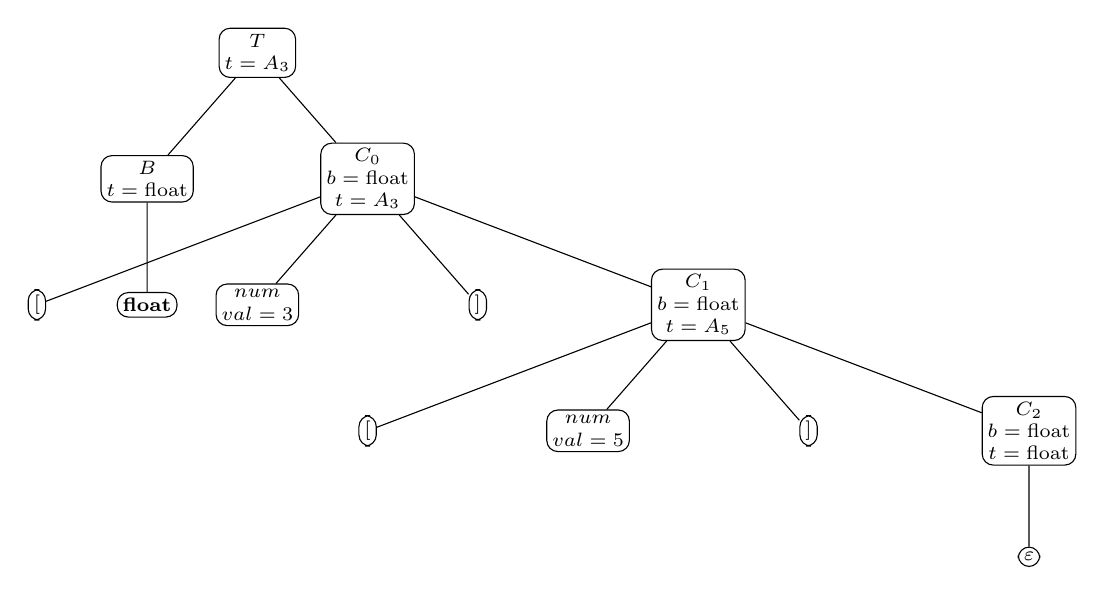
\begin{tikzpicture}[
    level distance=16mm,
    sibling distance=28mm,
    every node/.style={draw,rounded corners,align=center,font=\scriptsize,inner sep=2pt},
    edge from parent/.style={draw,-}
]
\node {$T$\\$t=A_3$}
    child {
        node {$B$\\$t=\mathrm{float}$}
        child { node {$\mathbf{float}$} }
    }
    child {
        node {$C_0$\\$b=\mathrm{float}$\\$t=A_3$}
        child { node {$[$} }
        child { node {$num$\\$val=3$} }
        child { node {$]$} }
        child {
            node {$C_1$\\$b=\mathrm{float}$\\$t=A_5$}
            child { node {$[$} }
            child { node {$num$\\$val=5$} }
            child { node {$]$} }
            child {
                node {$C_2$\\$b=\mathrm{float}$\\$t=\mathrm{float}$}
                child { node {$\varepsilon$} }
            }
        }
    };
\end{tikzpicture}
\end{center}

因此，输入串 \texttt{float[3][5]} 对应的最终类型为：
\[
T.t=\mathrm{array}(3,\mathrm{array}(5,\mathrm{float})).
\]

\section*{第 4 题}

根据题图，语言的表达式形式为：
\[
\begin{array}{rcl}
Expr &\to& \mathbf{for}\ id := int_1\ \mathbf{to}\ int_2\ \mathbf{do}\ Expr_1 \\
&\mid& id := Expr_1 \\
&\mid& Expr_1 ; Expr_2 \\
&\mid& Expr_1 * Expr_2 \\
&\mid& Expr_1 + Expr_2 \\
&\mid& id \\
&\mid& int
\end{array}
\]

下面假设 \textbf{for-to} 循环上下界合法，且循环次数按闭区间计算：
\[
n=int_2.val-int_1.val+1.
\]

\subsection*{(1) 计算开销函数的 SDD}

为每个 $Expr$ 设置属性 $cp$ 表示该表达式的开销。终结符 $int$ 带有词法属性 $val$。

\[
\begin{array}{rcl}
Expr &\to& \mathbf{for}\ id := int_1\ \mathbf{to}\ int_2\ \mathbf{do}\ Expr_1 \\
\multicolumn{3}{l}{\qquad Expr.cp=3+(int_2.val-int_1.val+1)\times Expr_1.cp} \\[1mm]
Expr &\to& id := Expr_1 \\
\multicolumn{3}{l}{\qquad Expr.cp=1+Expr_1.cp} \\[1mm]
Expr &\to& Expr_1 ; Expr_2 \\
\multicolumn{3}{l}{\qquad Expr.cp=Expr_1.cp+Expr_2.cp} \\[1mm]
Expr &\to& Expr_1 * Expr_2 \\
\multicolumn{3}{l}{\qquad Expr.cp=2+Expr_1.cp+Expr_2.cp} \\[1mm]
Expr &\to& Expr_1 + Expr_2 \\
\multicolumn{3}{l}{\qquad Expr.cp=1+Expr_1.cp+Expr_2.cp} \\[1mm]
Expr &\to& id \\
\multicolumn{3}{l}{\qquad Expr.cp=1} \\[1mm]
Expr &\to& int \\
\multicolumn{3}{l}{\qquad Expr.cp=1}
\end{array}
\]

说明：
\begin{itemize}
    \item 顺序操作本身开销为 $0$，因此只累加两个子表达式的开销。
    \item 赋值操作的开销为 $1$，并累加右值表达式 $Expr_1$ 的开销；左部 $id$ 不是作为普通变量表达式参与求值，因此不额外加 $id$ 的表达式开销。
    \item 循环操作本身开销为 $3$，循环体 $Expr_1$ 的开销乘以循环次数。
\end{itemize}

\subsection*{(2) 属性分类}

本 SDD 中引入的属性如下：

\begin{center}
\begin{tabular}{|c|p{10cm}|}
\hline
属性 & 类型与理由 \\
\hline
$Expr.cp$ & 综合属性。它总是在产生式左部的 $Expr$ 上被定义，并由右部子表达式的 $cp$、终结符的词法值或常量计算得到。 \\
\hline
$int.val$ & 终结符的综合属性。它由词法分析器给出，用于计算循环次数。 \\
\hline
\end{tabular}
\end{center}

该定义中没有引入继承属性。

\end{document}
